% Options for packages loaded elsewhere
\PassOptionsToPackage{unicode}{hyperref}
\PassOptionsToPackage{hyphens}{url}
\PassOptionsToPackage{dvipsnames,svgnames,x11names}{xcolor}
%
\documentclass[
  12pt,
]{book}
\usepackage{amsmath,amssymb}
\usepackage{lmodern}
\usepackage{setspace}
\usepackage{iftex}
\ifPDFTeX
  \usepackage[T1]{fontenc}
  \usepackage[utf8]{inputenc}
  \usepackage{textcomp} % provide euro and other symbols
\else % if luatex or xetex
  \usepackage{unicode-math}
  \defaultfontfeatures{Scale=MatchLowercase}
  \defaultfontfeatures[\rmfamily]{Ligatures=TeX,Scale=1}
\fi
% Use upquote if available, for straight quotes in verbatim environments
\IfFileExists{upquote.sty}{\usepackage{upquote}}{}
\IfFileExists{microtype.sty}{% use microtype if available
  \usepackage[]{microtype}
  \UseMicrotypeSet[protrusion]{basicmath} % disable protrusion for tt fonts
}{}
\makeatletter
\@ifundefined{KOMAClassName}{% if non-KOMA class
  \IfFileExists{parskip.sty}{%
    \usepackage{parskip}
  }{% else
    \setlength{\parindent}{0pt}
    \setlength{\parskip}{6pt plus 2pt minus 1pt}}
}{% if KOMA class
  \KOMAoptions{parskip=half}}
\makeatother
\usepackage{xcolor}
\usepackage[top=1in,left=1in,right=1in,bottom=1in]{geometry}
\usepackage{color}
\usepackage{fancyvrb}
\newcommand{\VerbBar}{|}
\newcommand{\VERB}{\Verb[commandchars=\\\{\}]}
\DefineVerbatimEnvironment{Highlighting}{Verbatim}{commandchars=\\\{\}}
% Add ',fontsize=\small' for more characters per line
\usepackage{framed}
\definecolor{shadecolor}{RGB}{248,248,248}
\newenvironment{Shaded}{\begin{snugshade}}{\end{snugshade}}
\newcommand{\AlertTok}[1]{\textcolor[rgb]{0.94,0.16,0.16}{#1}}
\newcommand{\AnnotationTok}[1]{\textcolor[rgb]{0.56,0.35,0.01}{\textbf{\textit{#1}}}}
\newcommand{\AttributeTok}[1]{\textcolor[rgb]{0.77,0.63,0.00}{#1}}
\newcommand{\BaseNTok}[1]{\textcolor[rgb]{0.00,0.00,0.81}{#1}}
\newcommand{\BuiltInTok}[1]{#1}
\newcommand{\CharTok}[1]{\textcolor[rgb]{0.31,0.60,0.02}{#1}}
\newcommand{\CommentTok}[1]{\textcolor[rgb]{0.56,0.35,0.01}{\textit{#1}}}
\newcommand{\CommentVarTok}[1]{\textcolor[rgb]{0.56,0.35,0.01}{\textbf{\textit{#1}}}}
\newcommand{\ConstantTok}[1]{\textcolor[rgb]{0.00,0.00,0.00}{#1}}
\newcommand{\ControlFlowTok}[1]{\textcolor[rgb]{0.13,0.29,0.53}{\textbf{#1}}}
\newcommand{\DataTypeTok}[1]{\textcolor[rgb]{0.13,0.29,0.53}{#1}}
\newcommand{\DecValTok}[1]{\textcolor[rgb]{0.00,0.00,0.81}{#1}}
\newcommand{\DocumentationTok}[1]{\textcolor[rgb]{0.56,0.35,0.01}{\textbf{\textit{#1}}}}
\newcommand{\ErrorTok}[1]{\textcolor[rgb]{0.64,0.00,0.00}{\textbf{#1}}}
\newcommand{\ExtensionTok}[1]{#1}
\newcommand{\FloatTok}[1]{\textcolor[rgb]{0.00,0.00,0.81}{#1}}
\newcommand{\FunctionTok}[1]{\textcolor[rgb]{0.00,0.00,0.00}{#1}}
\newcommand{\ImportTok}[1]{#1}
\newcommand{\InformationTok}[1]{\textcolor[rgb]{0.56,0.35,0.01}{\textbf{\textit{#1}}}}
\newcommand{\KeywordTok}[1]{\textcolor[rgb]{0.13,0.29,0.53}{\textbf{#1}}}
\newcommand{\NormalTok}[1]{#1}
\newcommand{\OperatorTok}[1]{\textcolor[rgb]{0.81,0.36,0.00}{\textbf{#1}}}
\newcommand{\OtherTok}[1]{\textcolor[rgb]{0.56,0.35,0.01}{#1}}
\newcommand{\PreprocessorTok}[1]{\textcolor[rgb]{0.56,0.35,0.01}{\textit{#1}}}
\newcommand{\RegionMarkerTok}[1]{#1}
\newcommand{\SpecialCharTok}[1]{\textcolor[rgb]{0.00,0.00,0.00}{#1}}
\newcommand{\SpecialStringTok}[1]{\textcolor[rgb]{0.31,0.60,0.02}{#1}}
\newcommand{\StringTok}[1]{\textcolor[rgb]{0.31,0.60,0.02}{#1}}
\newcommand{\VariableTok}[1]{\textcolor[rgb]{0.00,0.00,0.00}{#1}}
\newcommand{\VerbatimStringTok}[1]{\textcolor[rgb]{0.31,0.60,0.02}{#1}}
\newcommand{\WarningTok}[1]{\textcolor[rgb]{0.56,0.35,0.01}{\textbf{\textit{#1}}}}
\usepackage{longtable,booktabs,array}
\usepackage{calc} % for calculating minipage widths
% Correct order of tables after \paragraph or \subparagraph
\usepackage{etoolbox}
\makeatletter
\patchcmd\longtable{\par}{\if@noskipsec\mbox{}\fi\par}{}{}
\makeatother
% Allow footnotes in longtable head/foot
\IfFileExists{footnotehyper.sty}{\usepackage{footnotehyper}}{\usepackage{footnote}}
\makesavenoteenv{longtable}
\usepackage{graphicx}
\makeatletter
\def\maxwidth{\ifdim\Gin@nat@width>\linewidth\linewidth\else\Gin@nat@width\fi}
\def\maxheight{\ifdim\Gin@nat@height>\textheight\textheight\else\Gin@nat@height\fi}
\makeatother
% Scale images if necessary, so that they will not overflow the page
% margins by default, and it is still possible to overwrite the defaults
% using explicit options in \includegraphics[width, height, ...]{}
\setkeys{Gin}{width=\maxwidth,height=\maxheight,keepaspectratio}
% Set default figure placement to htbp
\makeatletter
\def\fps@figure{htbp}
\makeatother
\setlength{\emergencystretch}{3em} % prevent overfull lines
\providecommand{\tightlist}{%
  \setlength{\itemsep}{0pt}\setlength{\parskip}{0pt}}
\setcounter{secnumdepth}{5}

% English
\usepackage{booktabs}
\usepackage{longtable}
\makeatletter
\def\thm@space@setup{%
  \thm@preskip=8pt plus 2pt minus 4pt
  \thm@postskip=\thm@preskip
}
\makeatother

% 中文
% \usepackage{ctex}
% \usepackage{amsthm,mathrsfs}
% \usepackage{booktabs}
% \usepackage{longtable}
% \makeatletter
% \def\thm@space@setup{%
%   \thm@preskip=8pt plus 2pt minus 4pt
%   \thm@postskip=\thm@preskip
% }
% \makeatother
\ifLuaTeX
  \usepackage{selnolig}  % disable illegal ligatures
\fi
\usepackage[]{natbib}
\bibliographystyle{apalike}
\IfFileExists{bookmark.sty}{\usepackage{bookmark}}{\usepackage{hyperref}}
\IfFileExists{xurl.sty}{\usepackage{xurl}}{} % add URL line breaks if available
\urlstyle{same} % disable monospaced font for URLs
\hypersetup{
  pdftitle={The Principle of R Package GSClassifier},
  pdfauthor={Weibin Huang},
  colorlinks=true,
  linkcolor={blue},
  filecolor={Maroon},
  citecolor={Blue},
  urlcolor={Blue},
  pdfcreator={LaTeX via pandoc}}

\title{The Principle of R Package GSClassifier}
\author{Weibin Huang}
\date{2022-09-15}

\begin{document}
\maketitle

{
\hypersetup{linkcolor=}
\setcounter{tocdepth}{2}
\tableofcontents
}
\setstretch{1.5}
\hypertarget{the-principle-of-gsclassifier}{%
\chapter{The Principle of GSClassifier}\label{the-principle-of-gsclassifier}}

\hypertarget{introduction}{%
\section{Introduction}\label{introduction}}

\href{https://github.com/huangwb8/GSClassifier}{GSClassifier} is an R package for modeling and identification of Gene Expression Profiles (GEPs) subtypes. The detail of \textbf{GSClassifier} package usage had been demonstrated in \href{https://github.com/huangwb8/GSClassifier/wiki}{Github WiKi}. Here, we propose to introduce the principle of GSClassifier, including flowchart, \textbf{top scoring pairs (TSP)} algorithm, and batch effect control.

\hypertarget{flowchart}{%
\section{Flowchart}\label{flowchart}}

The flowchart of \textbf{GSClassifier} is showed in Figure \ref{fig:flowchart}.

\begin{figure}

{\centering 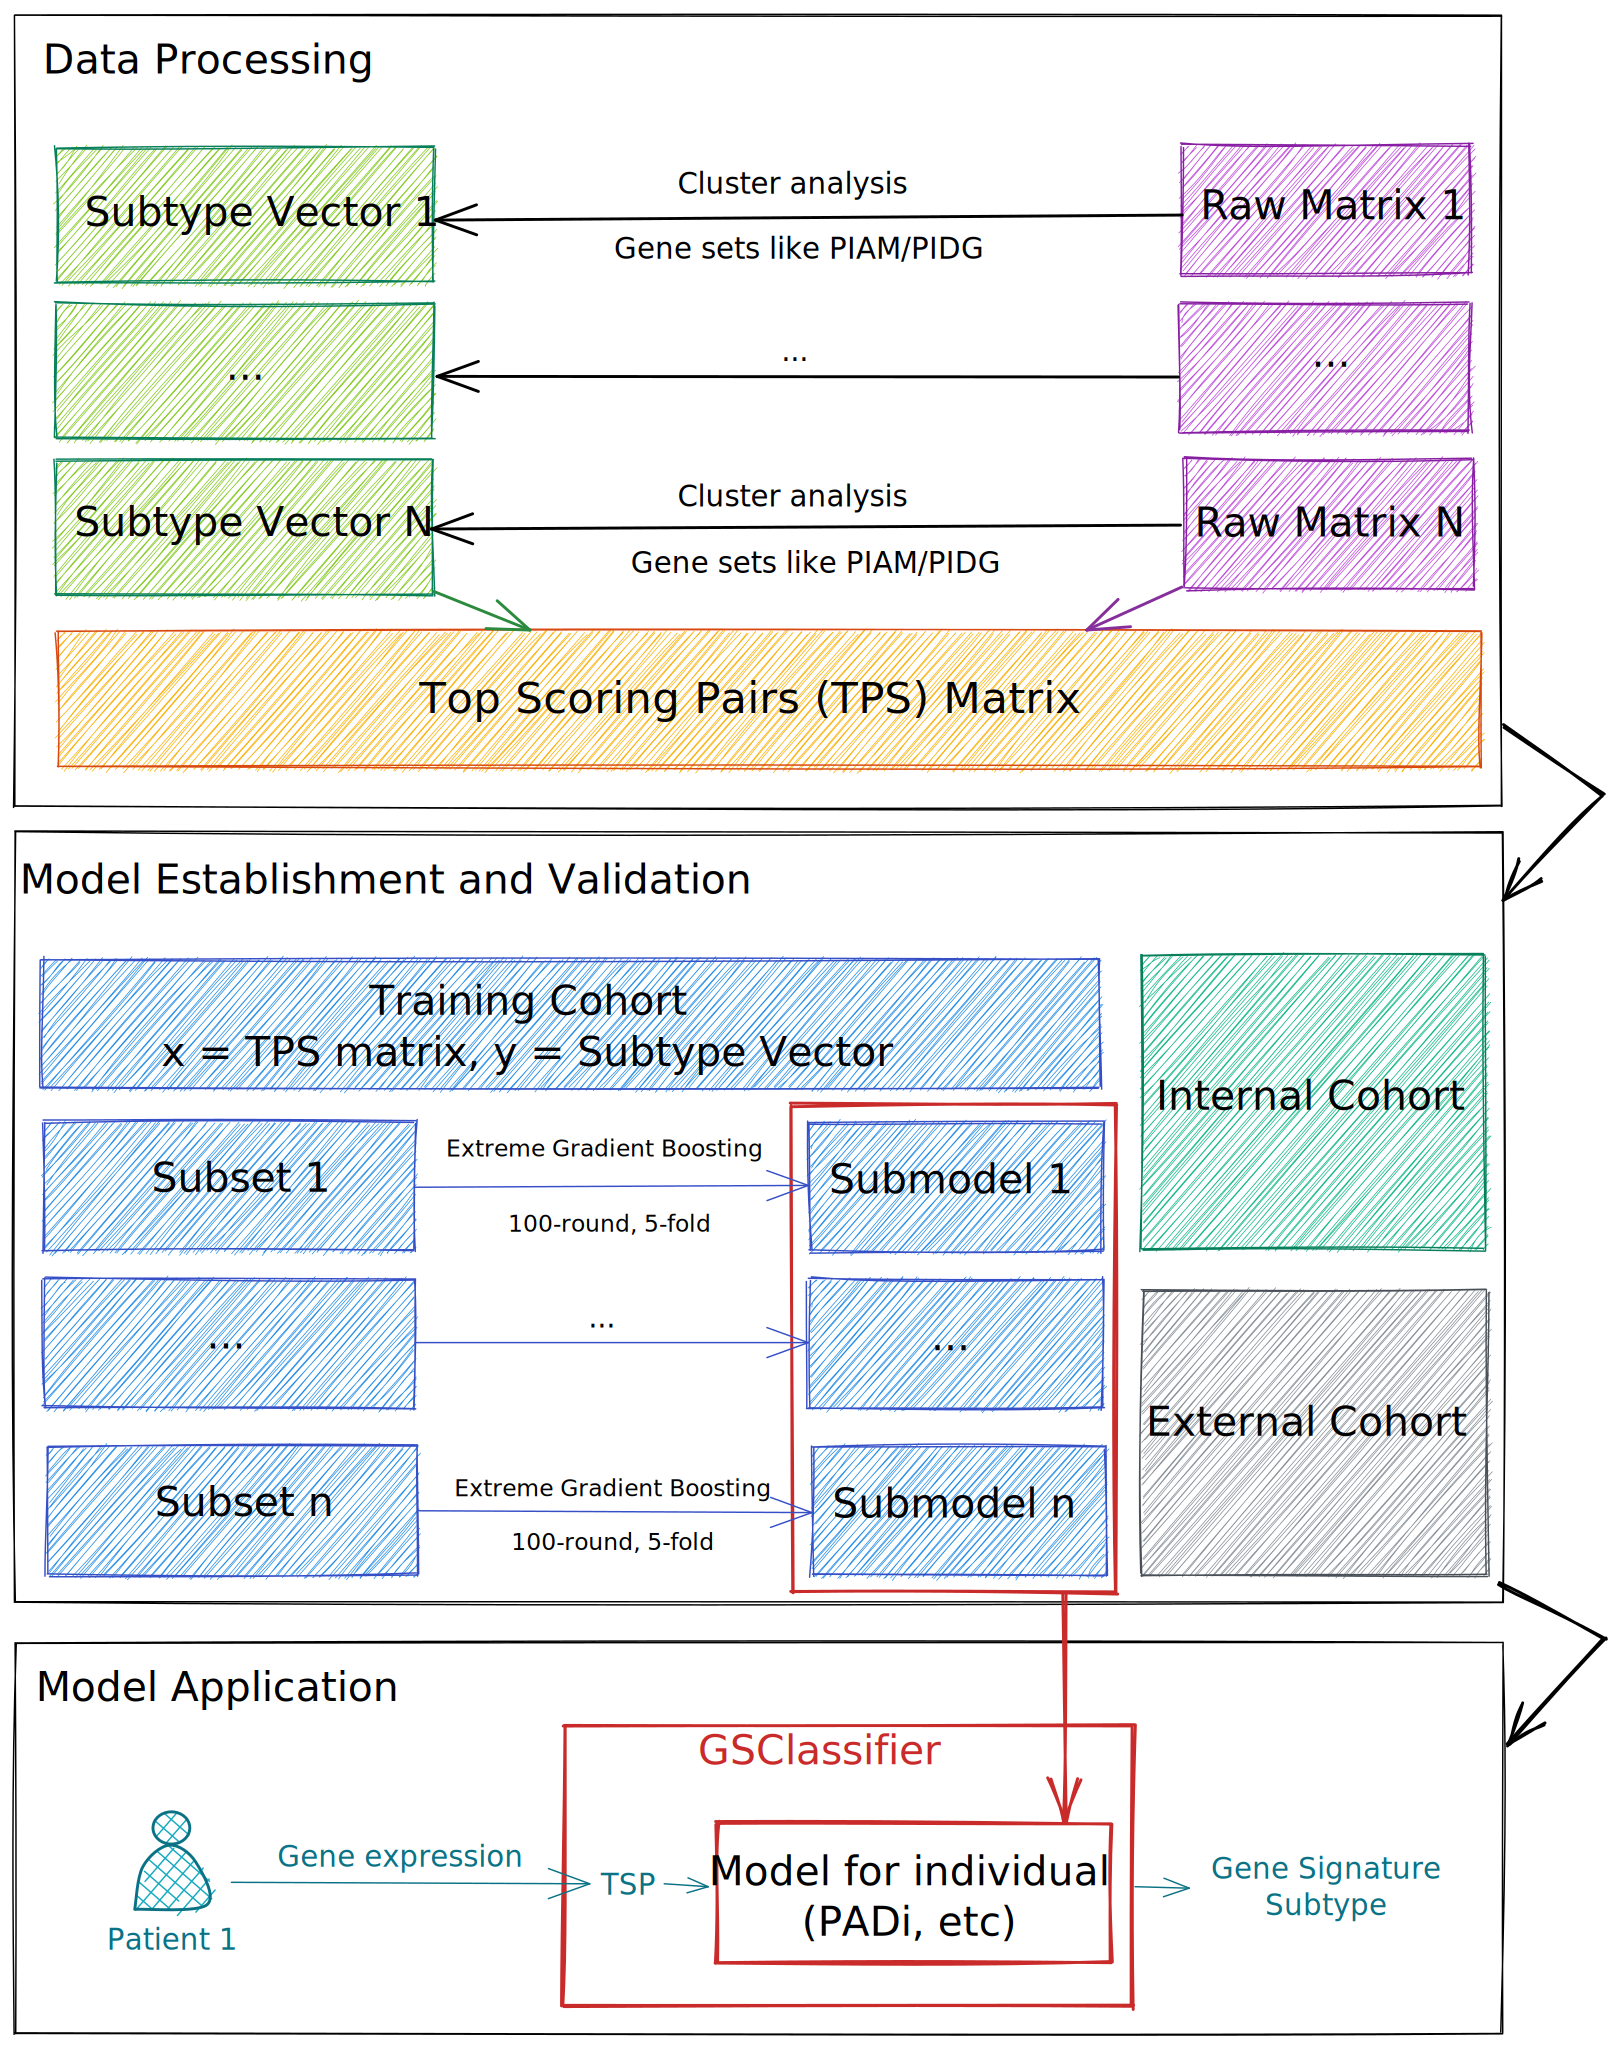
\includegraphics[width=0.9\linewidth]{./fig/flowchart} 

}

\caption{The flow chart of GSClassifier}\label{fig:flowchart}
\end{figure}

\hypertarget{data-processing}{%
\subsection{Data Processing}\label{data-processing}}

For each dataset, RNA expression matrix would be normalized internally (\textbf{Raw Matrix}) so that the expression data of the samples in the dataset were comparable and suitable for subtype identification. As demonstrated in Figure \ref{fig:flowchart}, the \textbf{Subtype vector} is identified based on independent cohorts instead of a merged matrix with batch effect control technologies. More details about batch effect control are discussed in \ref{subtypevector}.

There is no standard method to figure out subtype vectors. It depends on the Gene Expression Profiles (GEPs) used, the biological problems or ideas of researchers. For \textbf{Pan-immune Activation and Dysfunction (PAD)} subtypes, the GEPs, \textbf{Pan-Immune Activation Module (PIAM)} and \textbf{Pan-Immune Dysfunction Genes (PIDG)}, are biologically associated and suitable for calling four sutbypes (PIAM\textsuperscript{high}PIDG\textsuperscript{high}, PIAM\textsuperscript{high}PIDG\textsuperscript{low}, PIAM\textsuperscript{low}PIDG\textsuperscript{high}, and PIAM\textsuperscript{low}PIDG\textsuperscript{low}). Theoretically, we can also use a category strategy like low/medium/high, but more evidences or motivations are lacked for chasing such a complex model.

With subtype vectors and raw matrices, \textbf{Top Scoring Pairs (TSP)}, the core data format for model training and application in GSClassifier, would be calculated for the following process. The details of TSP are summarized in \ref{topicTSP}.

\hypertarget{model-establishment-and-validation}{%
\subsection{Model Establishment and Validation}\label{model-establishment-and-validation}}

The TSP matrix would be devided into training cohort and internal validation cohort. In PAD project, the rate of samples (training vs.~test) is \textbf{7:3}. Next, each \textbf{Subset} (70\% of the training cohort in PAD project) would be further selected randomly to build a \textbf{Submodel} via cross-validation Extreme Gradient Boosting algorithm (\textbf{xgboost::xgb.cv} function),. The number of submodels is suggested over 20 (more details in \ref{topicSubmodel}).

The internal validation cohort and external validation cohort (if any) would be used to test the performace of the trained model. By the way, \textbf{the data of both internal and external validation cohort would not be used during model training}.

\hypertarget{model-application}{%
\subsection{Model Application}\label{model-application}}

In PAD project, \textbf{Model for individual}, the ensemble of submodels, is called ``\textbf{PAD for individual}'' (\textbf{PADi}). Supposed raw RNA expression of a patient was given, \textbf{GSClassifier} would turn it into TSP vector, which would be as a input to \textbf{PADi}. Then, \textbf{GSClassifier} would output the possibility matrix and the subtype for this patient. No extra data (RNA expression of others, follow-up data, etc) would be needed but RNA expression of the patient for subtype identification, so models like \textbf{PADi} are personalized.

\hypertarget{topicTSP}{%
\section{Top scoring pairs}\label{topicTSP}}

Genes expression of an individual is normalized during the model training and the subtype identification via \textbf{Top Scoring Pairs} (\textbf{TSP}) algorithm, which was previously described by Geman et al. TSP had been used in cancer research and effectively predicts cancer progression and ICIs response. Immuno-predictive score (IMPRES), a method resemble TSP, performed well in prediction of ICIs response in melanoma. Moreover, gene-pairing strategy was applied to reduce batch effect in several researches.

TSP normalization for an individual depends on its transcript data, implying that subtype calling would not be perturbed by data from other individuals or other extra information like follow-up data. As show in Figure \ref{fig:tsp}, The TSP matrix in GSClassifier consists of 3 parts: \textbf{binned expression}, \textbf{pair difference}, and \textbf{set difference}. In this section, we would conduct some experiments to demonstrate the potential of TSP normalization for development of cross-dataset/platform GEP-based models.

\begin{figure}

{\centering \includegraphics[width=0.85\linewidth]{./fig/TSP} 

}

\caption{The components of TSP (2 gene sets)}\label{fig:tsp}
\end{figure}

\hypertarget{packages}{%
\subsection{Packages}\label{packages}}

First, load needed packages:

\begin{Shaded}
\begin{Highlighting}[]

\CommentTok{\# Install "devtools" package}
\ControlFlowTok{if}\NormalTok{ (}\SpecialCharTok{!}\FunctionTok{requireNamespace}\NormalTok{(}\StringTok{"devtools"}\NormalTok{, }\AttributeTok{quietly =} \ConstantTok{TRUE}\NormalTok{))}
  \FunctionTok{install.packages}\NormalTok{(}\StringTok{"devtools"}\NormalTok{)}

\CommentTok{\# Install dependencies}
\ControlFlowTok{if}\NormalTok{ (}\SpecialCharTok{!}\FunctionTok{requireNamespace}\NormalTok{(}\StringTok{"luckyBase"}\NormalTok{, }\AttributeTok{quietly =} \ConstantTok{TRUE}\NormalTok{))}
\NormalTok{  devtools}\SpecialCharTok{::}\FunctionTok{install\_github}\NormalTok{(}\StringTok{"huangwb8/luckyBase"}\NormalTok{)}

\CommentTok{\# Install the "GSClassifier" package}
\ControlFlowTok{if}\NormalTok{ (}\SpecialCharTok{!}\FunctionTok{requireNamespace}\NormalTok{(}\StringTok{"GSClassifier"}\NormalTok{, }\AttributeTok{quietly =} \ConstantTok{TRUE}\NormalTok{))}
\NormalTok{  devtools}\SpecialCharTok{::}\FunctionTok{install\_github}\NormalTok{(}\StringTok{"huangwb8/GSClassifier"}\NormalTok{)}

\CommentTok{\# Install the "pacman" package}
\ControlFlowTok{if}\NormalTok{ (}\SpecialCharTok{!}\FunctionTok{requireNamespace}\NormalTok{(}\StringTok{"pacman"}\NormalTok{, }\AttributeTok{quietly =} \ConstantTok{TRUE}\NormalTok{))\{}
  \FunctionTok{install.packages}\NormalTok{(}\StringTok{"pacman"}\NormalTok{)}
  \FunctionTok{library}\NormalTok{(pacman)}
\NormalTok{\} }\ControlFlowTok{else}\NormalTok{ \{}
  \FunctionTok{library}\NormalTok{(pacman)}
\NormalTok{\}}

\CommentTok{\# Load needed packages}
\NormalTok{packages\_needed }\OtherTok{\textless{}{-}} \FunctionTok{c}\NormalTok{(}
  \StringTok{"readxl"}\NormalTok{,}
  \StringTok{"ComplexHeatmap"}\NormalTok{,}
  \StringTok{"GSClassifier"}\NormalTok{,}
  \StringTok{"rpart"}\NormalTok{,}
  \StringTok{"tidyr"}\NormalTok{)}
\ControlFlowTok{for}\NormalTok{(i }\ControlFlowTok{in}\NormalTok{ packages\_needed)\{}\FunctionTok{p\_load}\NormalTok{(}\AttributeTok{char=}\NormalTok{i)\}}
\end{Highlighting}
\end{Shaded}

\hypertarget{simulated-dataset}{%
\subsection{Simulated Dataset}\label{simulated-dataset}}

We simulated a dataset to demonstrate the principle of TSP normalization in GSClassifier:

\begin{Shaded}
\begin{Highlighting}[]
\CommentTok{\# Geneset}
\NormalTok{geneSet }\OtherTok{\textless{}{-}} \FunctionTok{list}\NormalTok{(}
  \AttributeTok{Set1 =} \FunctionTok{paste}\NormalTok{(}\StringTok{\textquotesingle{}Gene\textquotesingle{}}\NormalTok{,}\DecValTok{1}\SpecialCharTok{:}\DecValTok{3}\NormalTok{,}\AttributeTok{sep =} \StringTok{\textquotesingle{}\textquotesingle{}}\NormalTok{),}
  \AttributeTok{Set2 =} \FunctionTok{paste}\NormalTok{(}\StringTok{\textquotesingle{}Gene\textquotesingle{}}\NormalTok{,}\DecValTok{4}\SpecialCharTok{:}\DecValTok{6}\NormalTok{,}\AttributeTok{sep =} \StringTok{\textquotesingle{}\textquotesingle{}}\NormalTok{)}
\NormalTok{)}

\CommentTok{\# RNA expression}
\NormalTok{x }\OtherTok{\textless{}{-}} \FunctionTok{read\_xlsx}\NormalTok{(}\StringTok{\textquotesingle{}./data/simulated{-}data.xlsx\textquotesingle{}}\NormalTok{, }\AttributeTok{sheet =} \StringTok{\textquotesingle{}RNA\textquotesingle{}}\NormalTok{)}
\NormalTok{expr0 }\OtherTok{\textless{}{-}} \FunctionTok{as.matrix}\NormalTok{(x[,}\SpecialCharTok{{-}}\DecValTok{1}\NormalTok{])}
\FunctionTok{rownames}\NormalTok{(expr0) }\OtherTok{\textless{}{-}} \FunctionTok{as.character}\NormalTok{(}\FunctionTok{as.matrix}\NormalTok{(x[,}\DecValTok{1}\NormalTok{])); }\FunctionTok{rm}\NormalTok{(x)}

\CommentTok{\# Subtype information}
\CommentTok{\# It depends on the application scenarios of GEPs}
\NormalTok{subtype\_vector }\OtherTok{\textless{}{-}} \FunctionTok{c}\NormalTok{(}\DecValTok{1}\NormalTok{, }\DecValTok{1}\NormalTok{, }\DecValTok{1}\NormalTok{, }\DecValTok{2}\NormalTok{, }\DecValTok{2}\NormalTok{, }\DecValTok{2}\NormalTok{)}
\CommentTok{\# Binned data for subtype 1}
\NormalTok{Ybin }\OtherTok{\textless{}{-}} \FunctionTok{ifelse}\NormalTok{(subtype\_vector }\SpecialCharTok{==} \DecValTok{1}\NormalTok{, }\DecValTok{1}\NormalTok{, }\DecValTok{0}\NormalTok{)}

\CommentTok{\# Parameters}
\NormalTok{breakVec }\OtherTok{=} \FunctionTok{c}\NormalTok{(}\DecValTok{0}\NormalTok{, }\FloatTok{0.25}\NormalTok{, }\FloatTok{0.5}\NormalTok{, }\FloatTok{0.75}\NormalTok{, }\FloatTok{1.0}\NormalTok{)}

\CommentTok{\# Report}
\FunctionTok{cat}\NormalTok{(}\FunctionTok{c}\NormalTok{(}\StringTok{\textquotesingle{}}\SpecialCharTok{\textbackslash{}n}\StringTok{\textquotesingle{}}\NormalTok{, }\StringTok{\textquotesingle{}Gene sets:\textquotesingle{}}\NormalTok{, }\StringTok{\textquotesingle{}}\SpecialCharTok{\textbackslash{}n}\StringTok{\textquotesingle{}}\NormalTok{))}
\FunctionTok{print}\NormalTok{(geneSet)}
\FunctionTok{cat}\NormalTok{(}\StringTok{\textquotesingle{}RNA expression:\textquotesingle{}}\NormalTok{, }\StringTok{\textquotesingle{}}\SpecialCharTok{\textbackslash{}n}\StringTok{\textquotesingle{}}\NormalTok{)}
\FunctionTok{print}\NormalTok{(expr0)}
\CommentTok{\# }
\CommentTok{\#  Gene sets: }
\CommentTok{\# $Set1}
\CommentTok{\# [1] "Gene1" "Gene2" "Gene3"}
\CommentTok{\# }
\CommentTok{\# $Set2}
\CommentTok{\# [1] "Gene4" "Gene5" "Gene6"}
\CommentTok{\# }
\CommentTok{\# RNA expression: }
\CommentTok{\#       Sample1 Sample2 Sample3 Sample4 Sample5 Sample6}
\CommentTok{\# Gene1    0.51    0.52    0.60    0.21    0.30    0.40}
\CommentTok{\# Gene2    0.52    0.54    0.58    0.22    0.31    0.35}
\CommentTok{\# Gene3    0.53    0.60    0.61      NA    0.29    0.30}
\CommentTok{\# Gene4    0.21    0.30    0.40    0.51    0.52    0.60}
\CommentTok{\# Gene5    0.22    0.31    0.35    0.52    0.54    0.58}
\CommentTok{\# Gene6    0.23    0.29    0.30    0.53      NA    0.61}
\CommentTok{\# Gene7    0.10    0.12    0.09    0.11    0.12    0.14}
\end{Highlighting}
\end{Shaded}

Look at the matrix via heatmap:

\begin{Shaded}
\begin{Highlighting}[]
\FunctionTok{Heatmap}\NormalTok{(}\FunctionTok{t}\NormalTok{(}\FunctionTok{scale}\NormalTok{(}\FunctionTok{t}\NormalTok{(expr0))), }\AttributeTok{name =} \StringTok{"Z{-}score"}\NormalTok{)}
\end{Highlighting}
\end{Shaded}

\begin{center}\includegraphics[width=0.6\linewidth]{Flowchart_files/figure-latex/unnamed-chunk-3-1} \end{center}

This is an intersting dataset with features as following:

\begin{itemize}
\item
  \textbf{Distinguished gene sets}: The expression profile between \textbf{Gene 1-3} and \textbf{Gene 4-6} is obviously different arross samples. Thus, these gene sets might represent different biology meaning.
\item
  \textbf{Stable gene}: The expression level and rank of \textbf{Gene 7} seemed to be similar across samples. Thus, \textbf{Gene 7} might not be a robust marker for subtype modeling. Thus, it could help us to understand how filtering of \textbf{GSClassifier} works.
\item
  \textbf{Expression heterogeneity \& rank homogeneity}: Take \textbf{Sample1} and \textbf{Sample3} as examples. The expression of \textbf{Gene 1-6} in \textbf{Sample3} seemed to be higher than those of \textbf{Sample1}. However, the expression of \textbf{Gene 1-3} is higher than \textbf{Gene 4-6} in both \textbf{Sample1} and \textbf{Sample3}, indicating similar bioprocess in these samples exists so that they should be classified as the same subtype.
\end{itemize}

\hypertarget{missing-values}{%
\subsection{Missing values}\label{missing-values}}

Here, we fill missing value with Recursive Partitioning and Regression Trees (RPART) algorithm:

\begin{Shaded}
\begin{Highlighting}[]
\CommentTok{\# RPART}
\NormalTok{expr }\OtherTok{\textless{}{-}}\NormalTok{ GSClassifier}\SpecialCharTok{:::}\FunctionTok{na\_fill}\NormalTok{(expr0, }\AttributeTok{method=}\StringTok{"anova"}\NormalTok{, }\AttributeTok{na.action =}\NormalTok{ na.rpart)}

\CommentTok{\# Report}
\FunctionTok{cat}\NormalTok{(}\StringTok{\textquotesingle{}RNA expression:\textquotesingle{}}\NormalTok{, }\StringTok{\textquotesingle{}}\SpecialCharTok{\textbackslash{}n}\StringTok{\textquotesingle{}}\NormalTok{)}
\FunctionTok{print}\NormalTok{(expr0)}
\FunctionTok{cat}\NormalTok{(}\StringTok{\textquotesingle{}}\SpecialCharTok{\textbackslash{}n}\StringTok{\textquotesingle{}}\NormalTok{)}
\FunctionTok{cat}\NormalTok{(}\StringTok{\textquotesingle{}RNA expression without NA value:\textquotesingle{}}\NormalTok{, }\StringTok{\textquotesingle{}}\SpecialCharTok{\textbackslash{}n}\StringTok{\textquotesingle{}}\NormalTok{)}
\FunctionTok{print}\NormalTok{(expr)}
\CommentTok{\# RNA expression: }
\CommentTok{\#       Sample1 Sample2 Sample3 Sample4 Sample5 Sample6}
\CommentTok{\# Gene1    0.51    0.52    0.60    0.21    0.30    0.40}
\CommentTok{\# Gene2    0.52    0.54    0.58    0.22    0.31    0.35}
\CommentTok{\# Gene3    0.53    0.60    0.61      NA    0.29    0.30}
\CommentTok{\# Gene4    0.21    0.30    0.40    0.51    0.52    0.60}
\CommentTok{\# Gene5    0.22    0.31    0.35    0.52    0.54    0.58}
\CommentTok{\# Gene6    0.23    0.29    0.30    0.53      NA    0.61}
\CommentTok{\# Gene7    0.10    0.12    0.09    0.11    0.12    0.14}
\CommentTok{\# }
\CommentTok{\# RNA expression without NA value: }
\CommentTok{\#       Sample1 Sample2 Sample3 Sample4 Sample5 Sample6}
\CommentTok{\# Gene1    0.51    0.52    0.60   0.210   0.300    0.40}
\CommentTok{\# Gene2    0.52    0.54    0.58   0.220   0.310    0.35}
\CommentTok{\# Gene3    0.53    0.60    0.61   0.466   0.290    0.30}
\CommentTok{\# Gene4    0.21    0.30    0.40   0.510   0.520    0.60}
\CommentTok{\# Gene5    0.22    0.31    0.35   0.520   0.540    0.58}
\CommentTok{\# Gene6    0.23    0.29    0.30   0.530   0.392    0.61}
\CommentTok{\# Gene7    0.10    0.12    0.09   0.110   0.120    0.14}
\end{Highlighting}
\end{Shaded}

Look at the new matrix via heatmap, where the clustering result is not obviously disturbed by \textbf{NA} filling:

\begin{Shaded}
\begin{Highlighting}[]
\FunctionTok{Heatmap}\NormalTok{(}\FunctionTok{t}\NormalTok{(}\FunctionTok{scale}\NormalTok{(}\FunctionTok{t}\NormalTok{(expr))), }\AttributeTok{name =} \StringTok{"Z{-}score"}\NormalTok{)}
\end{Highlighting}
\end{Shaded}

\begin{center}\includegraphics[width=0.6\linewidth]{Flowchart_files/figure-latex/unnamed-chunk-5-1} \end{center}

Although RPART algorithm is proved to be powerful dealing with NA value, we should try to use markers with less NA as possible. During PAD subtype establishment, only genes occurring in over 80\% of datasets were retained so as to minumize the impact from mising value.

With \textbf{subtype vectors} and \textbf{Raw Matrix}, the TSP matrix for a specified subtypes could be calculated via function \texttt{GSClassifier::trainDataProc}:

\begin{Shaded}
\begin{Highlighting}[]
\FunctionTok{trainDataProc}\NormalTok{(}
\NormalTok{  Xmat, Yvec,}
  
\NormalTok{  geneSet, }

  \AttributeTok{subtype =} \DecValTok{1}\NormalTok{, }
  
  \CommentTok{\# 0.2 was Used in PAD project}
  \AttributeTok{ptail =} \FloatTok{0.2}\NormalTok{,}
  
  \CommentTok{\# c(0, 0.25, 0.5, 0.75, 1.0) was Used in PAD project}
  \AttributeTok{breakVec =} \FunctionTok{c}\NormalTok{(}\DecValTok{0}\NormalTok{, }\FloatTok{0.25}\NormalTok{, }\FloatTok{0.5}\NormalTok{, }\FloatTok{0.75}\NormalTok{, }\FloatTok{1.0}\NormalTok{)}
\NormalTok{)}
\end{Highlighting}
\end{Shaded}

\hypertarget{binned-expression}{%
\subsection{Binned expression}\label{binned-expression}}

First, we binned genes with diffrent quantile intervals so that the distribution of rank information could be more consistent across samples.

Take \textbf{Sample4} as an example:

\begin{Shaded}
\begin{Highlighting}[]

\CommentTok{\# Data of Sample4}

\NormalTok{x }\OtherTok{\textless{}{-}}\NormalTok{ expr[,}\DecValTok{4}\NormalTok{]}

\CommentTok{\# Create quantiles  }
\NormalTok{brks }\OtherTok{\textless{}{-}} \FunctionTok{quantile}\NormalTok{(}\FunctionTok{as.numeric}\NormalTok{(x), }
                 \AttributeTok{probs=}\NormalTok{breakVec, }
                 \AttributeTok{na.rm =}\NormalTok{ T)}

\CommentTok{\# Get interval orders}
\NormalTok{xbin }\OtherTok{\textless{}{-}} \FunctionTok{.bincode}\NormalTok{(}\AttributeTok{x =}\NormalTok{ x, }
                 \AttributeTok{breaks =}\NormalTok{ brks, }
                 \AttributeTok{include.lowest =}\NormalTok{ T)}
\NormalTok{xbin }\OtherTok{\textless{}{-}} \FunctionTok{as.numeric}\NormalTok{(xbin)}
\FunctionTok{names}\NormalTok{(xbin) }\OtherTok{\textless{}{-}} \FunctionTok{names}\NormalTok{(x)}

\CommentTok{\# Report}
\FunctionTok{cat}\NormalTok{(}\StringTok{\textquotesingle{}Quantiles:\textquotesingle{}}\NormalTok{, }\StringTok{\textquotesingle{}}\SpecialCharTok{\textbackslash{}n}\StringTok{\textquotesingle{}}\NormalTok{); }\FunctionTok{print}\NormalTok{(brks)}
\FunctionTok{cat}\NormalTok{(}\StringTok{\textquotesingle{}}\SpecialCharTok{\textbackslash{}n}\StringTok{\textquotesingle{}}\NormalTok{)}
\FunctionTok{cat}\NormalTok{(}\StringTok{\textquotesingle{}Raw expression:\textquotesingle{}}\NormalTok{, }\StringTok{\textquotesingle{}}\SpecialCharTok{\textbackslash{}n}\StringTok{\textquotesingle{}}\NormalTok{);}\FunctionTok{print}\NormalTok{(x)}
\FunctionTok{cat}\NormalTok{(}\StringTok{\textquotesingle{}}\SpecialCharTok{\textbackslash{}n}\StringTok{\textquotesingle{}}\NormalTok{)}
\FunctionTok{cat}\NormalTok{(}\StringTok{\textquotesingle{}Binned expression:\textquotesingle{}}\NormalTok{, }\StringTok{\textquotesingle{}}\SpecialCharTok{\textbackslash{}n}\StringTok{\textquotesingle{}}\NormalTok{); }\FunctionTok{print}\NormalTok{(xbin)}
\CommentTok{\# Quantiles: }
\CommentTok{\#    0\%   25\%   50\%   75\%  100\% }
\CommentTok{\# 0.110 0.215 0.466 0.515 0.530 }
\CommentTok{\# }
\CommentTok{\# Raw expression: }
\CommentTok{\# Gene1 Gene2 Gene3 Gene4 Gene5 Gene6 Gene7 }
\CommentTok{\# 0.210 0.220 0.466 0.510 0.520 0.530 0.110 }
\CommentTok{\# }
\CommentTok{\# Binned expression: }
\CommentTok{\# Gene1 Gene2 Gene3 Gene4 Gene5 Gene6 Gene7 }
\CommentTok{\#     1     2     2     3     4     4     1}
\end{Highlighting}
\end{Shaded}

For example, \textbf{0.110} is the minimun of the raw expression vector, so its binned expression is \textbf{1}. Similarly, the binned expression of maximum \textbf{0.530} is \textbf{4}.

Generally, we calculate binned expression via function \textbf{breakBin} of \textbf{GSClassifier}:

\begin{Shaded}
\begin{Highlighting}[]
\NormalTok{expr\_binned }\OtherTok{\textless{}{-}} \FunctionTok{apply}\NormalTok{(}
\NormalTok{  expr, }\DecValTok{2}\NormalTok{, }
\NormalTok{  GSClassifier}\SpecialCharTok{:::}\NormalTok{breakBin,}
\NormalTok{  breakVec)}
\FunctionTok{rownames}\NormalTok{(expr\_binned) }\OtherTok{\textless{}{-}} \FunctionTok{rownames}\NormalTok{(expr)}
\FunctionTok{print}\NormalTok{(expr\_binned)}
\CommentTok{\#       Sample1 Sample2 Sample3 Sample4 Sample5 Sample6}
\CommentTok{\# Gene1       3       3       4       1       2       2}
\CommentTok{\# Gene2       4       4       3       2       2       2}
\CommentTok{\# Gene3       4       4       4       2       1       1}
\CommentTok{\# Gene4       1       2       2       3       4       4}
\CommentTok{\# Gene5       2       2       2       4       4       3}
\CommentTok{\# Gene6       2       1       1       4       3       4}
\CommentTok{\# Gene7       1       1       1       1       1       1}
\end{Highlighting}
\end{Shaded}

In this simulated dataset, \textbf{Gene7} is a gene whose expression is always the lowest across all samples. In other words, the rank of \textbf{Gene7} is stable or invariable across samples so that it's not robust for identification of differentail subtypes.

Except binned expression, we also calculated pair difference later. Due to the number of gene pair is \(C_{2 \atop n}\), the removement of genes like \textbf{Gene7} before modeling could really reduce the complexibility and save computing resources. In all, genes with low rank difference should be dropped out in some extent in \textbf{GSClassifier}.

First, We use \textbf{base::rank} to return the sample ranks of the values in a vector:

\begin{Shaded}
\begin{Highlighting}[]
\NormalTok{expr\_binned\_rank }\OtherTok{\textless{}{-}} \FunctionTok{apply}\NormalTok{(}
\NormalTok{  expr\_binned, }\DecValTok{2}\NormalTok{, }
  \ControlFlowTok{function}\NormalTok{(x)}\FunctionTok{rank}\NormalTok{(x, }\AttributeTok{na.last =} \ConstantTok{TRUE}\NormalTok{)}
\NormalTok{)}
\FunctionTok{print}\NormalTok{(expr\_binned\_rank)}
\CommentTok{\#       Sample1 Sample2 Sample3 Sample4 Sample5 Sample6}
\CommentTok{\# Gene1     5.0     5.0     6.5     1.5     3.5     3.5}
\CommentTok{\# Gene2     6.5     6.5     5.0     3.5     3.5     3.5}
\CommentTok{\# Gene3     6.5     6.5     6.5     3.5     1.5     1.5}
\CommentTok{\# Gene4     1.5     3.5     3.5     5.0     6.5     6.5}
\CommentTok{\# Gene5     3.5     3.5     3.5     6.5     6.5     5.0}
\CommentTok{\# Gene6     3.5     1.5     1.5     6.5     5.0     6.5}
\CommentTok{\# Gene7     1.5     1.5     1.5     1.5     1.5     1.5}
\end{Highlighting}
\end{Shaded}

Then, get weighted average rank difference of each gene based on specified subtype distribution (\textbf{Ybin}):

\begin{Shaded}
\begin{Highlighting}[]
\NormalTok{testRes }\OtherTok{\textless{}{-}} \FunctionTok{sapply}\NormalTok{(}
  \DecValTok{1}\SpecialCharTok{:}\FunctionTok{nrow}\NormalTok{(expr\_binned\_rank), }
  \ControlFlowTok{function}\NormalTok{(gi)\{}
    
    \CommentTok{\# Rank vector of each gene}
\NormalTok{    rankg }\OtherTok{=}\NormalTok{ expr\_binned\_rank[gi,];}
    
    \CommentTok{\# Weighted average rank difference of a gene for specified subtype }
    \CommentTok{\# Here is subtype 1 vs. others}
\NormalTok{    (}\FunctionTok{sum}\NormalTok{(rankg[Ybin }\SpecialCharTok{==} \DecValTok{0}\NormalTok{], }\AttributeTok{na.rm =}\NormalTok{ T) }\SpecialCharTok{/} \FunctionTok{sum}\NormalTok{(Ybin }\SpecialCharTok{==} \DecValTok{0}\NormalTok{, }\AttributeTok{na.rm =}\NormalTok{ T)) }\SpecialCharTok{{-}} 
\NormalTok{    (}\FunctionTok{sum}\NormalTok{(rankg[Ybin }\SpecialCharTok{==} \DecValTok{1}\NormalTok{], }\AttributeTok{na.rm =}\NormalTok{ T) }\SpecialCharTok{/} \FunctionTok{sum}\NormalTok{(Ybin }\SpecialCharTok{==} \DecValTok{1}\NormalTok{, }\AttributeTok{na.rm =}\NormalTok{ T))}
\NormalTok{  \}}
\NormalTok{)}
\FunctionTok{names}\NormalTok{(testRes) }\OtherTok{\textless{}{-}} \FunctionTok{rownames}\NormalTok{(expr\_binned\_rank)}
\FunctionTok{print}\NormalTok{(testRes)}
\CommentTok{\#     Gene1     Gene2     Gene3     Gene4     Gene5     Gene6     Gene7 }
\CommentTok{\# {-}2.666667 {-}2.500000 {-}4.333333  3.166667  2.500000  3.833333  0.000000}
\end{Highlighting}
\end{Shaded}

\textbf{Gene7} is the one with the lowest absolute value (0) of rank diffrence. By the way, \textbf{Gene 1-3} have the same direction (\textless0), so do \textbf{Gene 4-6} (\textgreater0), which indicates the nature of clustering based on these two gene sets.

In practice, we use \textbf{ptail} to select differential genes based on rank diffrences. \textbf{Smaller ptail is, less gene kept}. Here, we just set \textbf{ptail=0.4}:

\begin{Shaded}
\begin{Highlighting}[]

\CommentTok{\# ptail is a numeber ranging (0,0.5].}
\NormalTok{ptail }\OtherTok{=} \FloatTok{0.4}

\CommentTok{\# Index of target genes with big rank differences}
\NormalTok{idx }\OtherTok{\textless{}{-}} \FunctionTok{which}\NormalTok{((testRes }\SpecialCharTok{\textless{}} \FunctionTok{quantile}\NormalTok{(testRes, ptail, }\AttributeTok{na.rm =}\NormalTok{ T)) }\SpecialCharTok{|} 
\NormalTok{             (testRes }\SpecialCharTok{\textgreater{}} \FunctionTok{quantile}\NormalTok{(testRes, }\FloatTok{1.0}\SpecialCharTok{{-}}\NormalTok{ptail, }\AttributeTok{na.rm =}\NormalTok{ T)))}

\CommentTok{\# Target genes}
\NormalTok{gene\_bigRank }\OtherTok{\textless{}{-}} \FunctionTok{names}\NormalTok{(testRes)[idx]}

\CommentTok{\# Report}
\FunctionTok{cat}\NormalTok{(}\StringTok{\textquotesingle{}Index of target genes: \textquotesingle{}}\NormalTok{,}\StringTok{\textquotesingle{}}\SpecialCharTok{\textbackslash{}n}\StringTok{\textquotesingle{}}\NormalTok{);}\FunctionTok{print}\NormalTok{(idx); }\FunctionTok{cat}\NormalTok{(}\StringTok{\textquotesingle{}}\SpecialCharTok{\textbackslash{}n}\StringTok{\textquotesingle{}}\NormalTok{)}
\FunctionTok{cat}\NormalTok{(}\StringTok{\textquotesingle{}Target genes:\textquotesingle{}}\NormalTok{,}\StringTok{\textquotesingle{}}\SpecialCharTok{\textbackslash{}n}\StringTok{\textquotesingle{}}\NormalTok{);}\FunctionTok{print}\NormalTok{(gene\_bigRank)}
\CommentTok{\# Index of target genes:  }
\CommentTok{\# Gene1 Gene2 Gene3 Gene4 Gene5 Gene6 }
\CommentTok{\#     1     2     3     4     5     6 }
\CommentTok{\# }
\CommentTok{\# Target genes: }
\CommentTok{\# [1] "Gene1" "Gene2" "Gene3" "Gene4" "Gene5" "Gene6"}
\end{Highlighting}
\end{Shaded}

Hence, \textbf{Gene7} was filtered and excluded in the following analysis. By the way, both \textbf{ptail} and \textbf{breakVec} are hyperparameters in GSClassifier modeling.

\hypertarget{pair-difference}{%
\subsection{Pair difference}\label{pair-difference}}

In GSClassifier, we use a ensemble function \textbf{featureSelection} to select data for pair difference scoring.

\begin{Shaded}
\begin{Highlighting}[]
\NormalTok{expr\_feat }\OtherTok{\textless{}{-}} \FunctionTok{featureSelection}\NormalTok{(expr, Ybin,}
                              \AttributeTok{testRes =}\NormalTok{ testRes,}
                              \AttributeTok{ptail =} \FloatTok{0.4}\NormalTok{)}

\NormalTok{expr\_sub }\OtherTok{\textless{}{-}}\NormalTok{ expr\_feat}\SpecialCharTok{$}\NormalTok{Xsub}
\NormalTok{gene\_bigRank }\OtherTok{\textless{}{-}}\NormalTok{ expr\_feat}\SpecialCharTok{$}\NormalTok{Genes}

\CommentTok{\# Report}
\FunctionTok{cat}\NormalTok{(}\StringTok{\textquotesingle{}Raw xpression without NA:\textquotesingle{}}\NormalTok{, }\StringTok{\textquotesingle{}}\SpecialCharTok{\textbackslash{}n}\StringTok{\textquotesingle{}}\NormalTok{)}
\FunctionTok{print}\NormalTok{(expr\_sub)}
\FunctionTok{cat}\NormalTok{(}\StringTok{\textquotesingle{}}\SpecialCharTok{\textbackslash{}n}\StringTok{\textquotesingle{}}\NormalTok{)}
\FunctionTok{cat}\NormalTok{(}\StringTok{\textquotesingle{}Genes with large rank diff:\textquotesingle{}}\NormalTok{, }\StringTok{\textquotesingle{}}\SpecialCharTok{\textbackslash{}n}\StringTok{\textquotesingle{}}\NormalTok{)}
\FunctionTok{print}\NormalTok{(gene\_bigRank)}
\CommentTok{\# Raw xpression without NA: }
\CommentTok{\#       Sample1 Sample2 Sample3 Sample4 Sample5 Sample6}
\CommentTok{\# Gene1    0.51    0.52    0.60   0.210   0.300    0.40}
\CommentTok{\# Gene2    0.52    0.54    0.58   0.220   0.310    0.35}
\CommentTok{\# Gene3    0.53    0.60    0.61   0.466   0.290    0.30}
\CommentTok{\# Gene4    0.21    0.30    0.40   0.510   0.520    0.60}
\CommentTok{\# Gene5    0.22    0.31    0.35   0.520   0.540    0.58}
\CommentTok{\# Gene6    0.23    0.29    0.30   0.530   0.392    0.61}
\CommentTok{\# }
\CommentTok{\# Genes with large rank diff: }
\CommentTok{\# [1] "Gene1" "Gene2" "Gene3" "Gene4" "Gene5" "Gene6"}
\end{Highlighting}
\end{Shaded}

In GSClassifier, we use function \textbf{makeGenePairs} to calculate s

\begin{Shaded}
\begin{Highlighting}[]
\NormalTok{gene\_bigRank\_pairs }\OtherTok{\textless{}{-}}\NormalTok{ GSClassifier}\SpecialCharTok{:::}\FunctionTok{makeGenePairs}\NormalTok{(}
\NormalTok{  gene\_bigRank, }
\NormalTok{  expr[gene\_bigRank,])}
\FunctionTok{print}\NormalTok{(gene\_bigRank\_pairs)}
\CommentTok{\#             Sample1 Sample2 Sample3 Sample4 Sample5 Sample6}
\CommentTok{\# Gene1:Gene2       0       0       1       0       0       1}
\CommentTok{\# Gene1:Gene3       0       0       0       0       1       1}
\CommentTok{\# Gene1:Gene4       1       1       1       0       0       0}
\CommentTok{\# Gene1:Gene5       1       1       1       0       0       0}
\CommentTok{\# Gene1:Gene6       1       1       1       0       0       0}
\CommentTok{\# Gene2:Gene3       0       0       0       0       1       1}
\CommentTok{\# Gene2:Gene4       1       1       1       0       0       0}
\CommentTok{\# Gene2:Gene5       1       1       1       0       0       0}
\CommentTok{\# Gene2:Gene6       1       1       1       0       0       0}
\CommentTok{\# Gene3:Gene4       1       1       1       0       0       0}
\CommentTok{\# Gene3:Gene5       1       1       1       0       0       0}
\CommentTok{\# Gene3:Gene6       1       1       1       0       0       0}
\CommentTok{\# Gene4:Gene5       0       0       1       0       0       1}
\CommentTok{\# Gene4:Gene6       0       1       1       0       1       0}
\CommentTok{\# Gene5:Gene6       0       1       1       0       1       0}
\end{Highlighting}
\end{Shaded}

Take \textbf{Gene1:Gene4} of \textbf{Sample1} as an example. \(Expression_{Gene1} - Expression_{Gene4} = 0.51-0.21 = 0.3 > 0\), so the pair score is 1. If the difference is less than or equal to 0, the pair score is 0. In addition, the difference of gene pair scoring between \textbf{Sample 1-3} and \textbf{Sample 4-6} is obivous, revealing the robustness of pair difference for subtype identification.

\hypertarget{set-difference}{%
\subsection{Set difference}\label{set-difference}}

In \textbf{GSClassifier}, \textbf{Set difference} is defined as a weight average of gene-geneset rank difference.

\begin{Shaded}
\begin{Highlighting}[]
\CommentTok{\# No. of gene sets}
\NormalTok{nGS }\OtherTok{=} \DecValTok{2}

\CommentTok{\# Name of gene set comparision, which is like s1s2, s1s3 and so on.}
\NormalTok{featureNames }\OtherTok{\textless{}{-}} \StringTok{\textquotesingle{}s1s2\textquotesingle{}}

\CommentTok{\# Gene set difference across samples}
\NormalTok{resultList }\OtherTok{\textless{}{-}} \FunctionTok{list}\NormalTok{()}
\ControlFlowTok{for}\NormalTok{ (i }\ControlFlowTok{in} \DecValTok{1}\SpecialCharTok{:}\FunctionTok{ncol}\NormalTok{(expr\_sub)) \{ }\CommentTok{\# i=1}
\NormalTok{  res0 }\OtherTok{\textless{}{-}} \FunctionTok{numeric}\NormalTok{(}\AttributeTok{length=}\FunctionTok{length}\NormalTok{(featureNames))}
\NormalTok{  idx }\OtherTok{\textless{}{-}} \DecValTok{1}
  \ControlFlowTok{for}\NormalTok{ (j1 }\ControlFlowTok{in} \DecValTok{1}\SpecialCharTok{:}\NormalTok{(nGS}\DecValTok{{-}1}\NormalTok{)) \{ }\CommentTok{\# j1=1}
    \ControlFlowTok{for}\NormalTok{ (j2 }\ControlFlowTok{in}\NormalTok{ (j1}\SpecialCharTok{+}\DecValTok{1}\NormalTok{)}\SpecialCharTok{:}\NormalTok{nGS) \{ }\CommentTok{\# j2=2}
      
      \CommentTok{\# If j1=1 and j2=2, gene sets s1/s2 would be selected}
      
      \CommentTok{\# Genes of different gene sets}
\NormalTok{      set1 }\OtherTok{\textless{}{-}}\NormalTok{ geneSet[[j1]] }\CommentTok{\# "Gene1" "Gene2" "Gene3"}
\NormalTok{      set2 }\OtherTok{\textless{}{-}}\NormalTok{ geneSet[[j2]] }\CommentTok{\# "Gene4" "Gene5" "Gene6"}
      
      \CommentTok{\# RNA expression of Genes by different gene sets}
\NormalTok{      vals1 }\OtherTok{\textless{}{-}}\NormalTok{ expr\_sub[}\FunctionTok{rownames}\NormalTok{(expr\_sub) }\SpecialCharTok{\%in\%}\NormalTok{ set1,i]}
      \CommentTok{\# Gene1 Gene2 Gene3}
      \CommentTok{\# 0.51  0.52  0.53}
\NormalTok{      vals2 }\OtherTok{\textless{}{-}}\NormalTok{ expr\_sub[}\FunctionTok{rownames}\NormalTok{(expr\_sub) }\SpecialCharTok{\%in\%}\NormalTok{ set2,i]}
      \CommentTok{\# Gene4 Gene5 Gene6}
      \CommentTok{\# 0.21  0.22  0.23}

      \CommentTok{\# Differences between one gene and gene sets}
      \CommentTok{\# Compare expression of each gene in Set1 with all genes in Set2. }
      \CommentTok{\# For example, 0.51\textgreater{}0.21/0.22/0.23, so the value of Gene1:s2 is 3.}
\NormalTok{      res1 }\OtherTok{\textless{}{-}} \FunctionTok{sapply}\NormalTok{(vals1, }\ControlFlowTok{function}\NormalTok{(v1) }\FunctionTok{sum}\NormalTok{(v1 }\SpecialCharTok{\textgreater{}}\NormalTok{ vals2, }\AttributeTok{na.rm=}\NormalTok{T))}
      \CommentTok{\# Gene1:s2   Gene2:s2   Gene3:s2}
      \CommentTok{\# 3          3           3}
      
      \CommentTok{\# Weight average of gene{-}geneset rank difference}
\NormalTok{      res0[idx] }\OtherTok{\textless{}{-}} \FunctionTok{sum}\NormalTok{(res1, }\AttributeTok{na.rm =}\NormalTok{ T) }\SpecialCharTok{/}\NormalTok{ (}\FunctionTok{length}\NormalTok{(vals1) }\SpecialCharTok{*} \FunctionTok{length}\NormalTok{(vals2))}
      
      \CommentTok{\# Next gene set pair}
\NormalTok{      idx }\OtherTok{\textless{}{-}}\NormalTok{ idx }\SpecialCharTok{+} \DecValTok{1}
\NormalTok{    \}}
\NormalTok{  \}}
\NormalTok{  resultList[[i]] }\OtherTok{\textless{}{-}} \FunctionTok{as.numeric}\NormalTok{(res0)}
\NormalTok{\}}
\NormalTok{resMat }\OtherTok{\textless{}{-}} \FunctionTok{do.call}\NormalTok{(cbind, resultList)}
\FunctionTok{colnames}\NormalTok{(resMat) }\OtherTok{\textless{}{-}} \FunctionTok{colnames}\NormalTok{(expr\_sub)}
\FunctionTok{rownames}\NormalTok{(resMat) }\OtherTok{\textless{}{-}}\NormalTok{ featureNames}

\CommentTok{\# Report }
\FunctionTok{cat}\NormalTok{(}\StringTok{\textquotesingle{}Set difference across samples: \textquotesingle{}}\NormalTok{, }\StringTok{\textquotesingle{}}\SpecialCharTok{\textbackslash{}n}\StringTok{\textquotesingle{}}\NormalTok{)}
\FunctionTok{print}\NormalTok{(resMat)}
\CommentTok{\# Set difference across samples:  }
\CommentTok{\#      Sample1 Sample2 Sample3 Sample4 Sample5 Sample6}
\CommentTok{\# s1s2       1       1       1       0       0       0}
\end{Highlighting}
\end{Shaded}

In \textbf{GSClassifier}, we established \textbf{makeSetData} to evaluate set difference across samples:

\begin{Shaded}
\begin{Highlighting}[]

\CommentTok{\# Gene set difference across samples}
\NormalTok{geneset\_interaction }\OtherTok{\textless{}{-}}\NormalTok{ GSClassifier}\SpecialCharTok{:::}\FunctionTok{makeSetData}\NormalTok{(expr\_sub, geneSet)}

\CommentTok{\# Report }
\FunctionTok{cat}\NormalTok{(}\StringTok{\textquotesingle{}Set difference across samples: \textquotesingle{}}\NormalTok{, }\StringTok{\textquotesingle{}}\SpecialCharTok{\textbackslash{}n}\StringTok{\textquotesingle{}}\NormalTok{)}
\FunctionTok{print}\NormalTok{(resMat)}
\CommentTok{\# Set difference across samples:  }
\CommentTok{\#      Sample1 Sample2 Sample3 Sample4 Sample5 Sample6}
\CommentTok{\# s1s2       1       1       1       0       0       0}
\end{Highlighting}
\end{Shaded}

We have known that the subtype of \textbf{Sample 1-3} differs from that of \textbf{Sample 4-6}, which revealed the robustness of set difference for subtype indentification.

As shown in Figure \ref{fig:tsp}, TSP matrix here should be :

\begin{Shaded}
\begin{Highlighting}[]

\CommentTok{\# TSP matrix}
\NormalTok{tsp }\OtherTok{\textless{}{-}} \FunctionTok{rbind}\NormalTok{(}
  
  \CommentTok{\# Binned expression}
\NormalTok{  expr\_binned[gene\_bigRank,],}
  
  \CommentTok{\# Pair difference}
\NormalTok{  gene\_bigRank\_pairs,}
  
  \CommentTok{\# Set difference}
\NormalTok{  resMat}
\NormalTok{)}

\CommentTok{\# Report }
\FunctionTok{cat}\NormalTok{(}\StringTok{\textquotesingle{}TSP matrix: \textquotesingle{}}\NormalTok{, }\StringTok{\textquotesingle{}}\SpecialCharTok{\textbackslash{}n}\StringTok{\textquotesingle{}}\NormalTok{)}
\FunctionTok{print}\NormalTok{(tsp)}
\CommentTok{\# TSP matrix:  }
\CommentTok{\#             Sample1 Sample2 Sample3 Sample4 Sample5 Sample6}
\CommentTok{\# Gene1             3       3       4       1       2       2}
\CommentTok{\# Gene2             4       4       3       2       2       2}
\CommentTok{\# Gene3             4       4       4       2       1       1}
\CommentTok{\# Gene4             1       2       2       3       4       4}
\CommentTok{\# Gene5             2       2       2       4       4       3}
\CommentTok{\# Gene6             2       1       1       4       3       4}
\CommentTok{\# Gene1:Gene2       0       0       1       0       0       1}
\CommentTok{\# Gene1:Gene3       0       0       0       0       1       1}
\CommentTok{\# Gene1:Gene4       1       1       1       0       0       0}
\CommentTok{\# Gene1:Gene5       1       1       1       0       0       0}
\CommentTok{\# Gene1:Gene6       1       1       1       0       0       0}
\CommentTok{\# Gene2:Gene3       0       0       0       0       1       1}
\CommentTok{\# Gene2:Gene4       1       1       1       0       0       0}
\CommentTok{\# Gene2:Gene5       1       1       1       0       0       0}
\CommentTok{\# Gene2:Gene6       1       1       1       0       0       0}
\CommentTok{\# Gene3:Gene4       1       1       1       0       0       0}
\CommentTok{\# Gene3:Gene5       1       1       1       0       0       0}
\CommentTok{\# Gene3:Gene6       1       1       1       0       0       0}
\CommentTok{\# Gene4:Gene5       0       0       1       0       0       1}
\CommentTok{\# Gene4:Gene6       0       1       1       0       1       0}
\CommentTok{\# Gene5:Gene6       0       1       1       0       1       0}
\CommentTok{\# s1s2              1       1       1       0       0       0}
\end{Highlighting}
\end{Shaded}

\hypertarget{discussion}{%
\chapter{Discussion}\label{discussion}}

\hypertarget{model-complexibility}{%
\section{Model complexibility}\label{model-complexibility}}

Linear growth/exponential growth

\hypertarget{missing-value}{%
\section{Missing value}\label{missing-value}}

Talk about strategy in subtypes modeling and calling

\hypertarget{extensibility}{%
\section{Extensibility}\label{extensibility}}

How could

\hypertarget{subtypevector}{%
\section{Subtype vector calling}\label{subtypevector}}

\hypertarget{topicSubmodel}{%
\section{The number of submodels}\label{topicSubmodel}}

Talk about the number of submodels we should train.

  \bibliography{book.bib,packages.bib}

\end{document}
